\documentclass[letterpaper,9pt,fleqn]{extarticle}
\usepackage[utf8]{inputenc}
\usepackage[T1]{fontenc}
\usepackage{graphicx}
\usepackage{xcolor}
\usepackage{tikz}
\usepackage{url}
\usepackage{qrcode}
\usetikzlibrary{shapes.geometric}
\usetikzlibrary{calc}
\usepackage{array}   % for \newcolumntype macro
%\usepackage{fourier}
\usepackage{graphicx,nicefrac}
\usepackage{isomath,upgreek,xcolor,comment,fourier}
\usepackage{pdfpages}
\usepackage{tkz-euclide}
%\usetkzobj{all}
\pagestyle{empty}
\usepackage[activate={true,nocompatibility},final,tracking=true,kerning=true,factor=1100,stretch=10,shrink=10]{microtype}
\usepackage[american]{babel}

\usepackage{amstext} % for \text macro
\usepackage{array}   % for \newcolumntype macro
\newcolumntype{L}{>{$}l<{$}} % math-mode version of "l" column type

\newcommand{\dom}{\mathrm{dom}} 
\newcommand{\range}{\mathrm{range}} 
\newcommand{\zero}{\mathrm{zero}} 
\newcommand{\reals}{\mathbf{R}} 
\newcommand{\integers}{\mathbf{Z}} 
\newcommand{\ssep}{\mid}
\newcommand{\arcsec}{\mathrm{arcsec}}
\newcommand{\arccsc}{\mathrm{arccsc}}
\newcommand{\arccot}{\mathrm{arccot}}

\usepackage{amsmath,amssymb,textcomp}
\everymath{\displaystyle}

%\usepackage{times}
%\renewcommand\familydefault{\sfdefault}
%\usepackage{tgheros}
%\usepackage[defaultmono,scale=0.85]{droidmono}
%\usepackage{fourier}
\usepackage{multicol}
\setlength{\columnseprule}{0pt}
\setlength{\columnsep}{20.0pt}


\usepackage{geometry}
\geometry{letterpaper,left=10mm,right=10mm,top=10mm,bottom=10mm}

\linespread{1.3}


% custom title
\makeatletter
\renewcommand*{\maketitle}{%
\noindent
\begin{minipage}{0.4\textwidth}

\begin{tikzpicture}
\node[rectangle,rounded corners=6pt,inner sep=10pt,fill=blue!50!black,text width= 0.95\textwidth] {\color{white}\Huge \@title};
\end{tikzpicture}
\end{minipage}
\hfill
\begin{minipage}{0.55\textwidth}

\begin{tikzpicture}
\node[rectangle,rounded corners=3pt,inner sep=10pt,draw=blue!50!black,text width= 0.95\textwidth] {\LARGE \@author};
\end{tikzpicture}
\end{minipage}
\bigskip\bigskip
}%
\makeatother

% custom section
\usepackage[explicit]{titlesec}
\newcommand*\sectionlabel{}
\titleformat{\section}
  {\gdef\sectionlabel{}
   \normalfont\sffamily\Large\bfseries\scshape}
  {\gdef\sectionlabel{\thesection\ }}{0pt}
  {
\noindent
\begin{tikzpicture}
\node[rectangle,rounded corners=3pt,inner sep=4pt,fill=blue!50!black,text width= 0.95\columnwidth] {\color{white}\sectionlabel#1};
\end{tikzpicture}
  }
\titlespacing*{\section}{0pt}{15pt}{10pt}


% custom footer
\usepackage{fancyhdr}
\makeatletter
%\pagestyle{fancy}
\fancyhead{}
%\fancyfoot[C]{\footnotesize \textcopyright\ \@date\ \ \@author}
\renewcommand{\headrulewidth}{0pt}
\renewcommand{\footrulewidth}{0pt}
\makeatother

\raggedbottom 
\allowdisplaybreaks
\usepackage{tikz-3dplot}
\begin{document}

%\maketitle

\begin{multicols*}{3}
  \raggedbottom 



\section*{Greek Characters}
\vspace{-0.35in}



\begin{tabular}{|L | L| L|} \hline
\mbox{Name} & \mbox{Symbol} & \mbox{Typical use(s)} \\ \hline
\mathrm{alpha} & \alpha  & \mbox{angle, constant} \\
\mathrm{beta} & \beta  & \mbox{angle, constant}  \\ 
\mathrm{gamma} & \gamma & \mbox{angle, constant} \\
\mathrm{delta} & \delta  & \mbox{limit definition}\\
\mathrm{epsilon} & \epsilon  \mbox{ or } \varepsilon & \mbox{limit definition} \\
\mathrm{theta}  & \theta  \mbox{ or } \vartheta &\mbox{angle}\\ 
%\mathrm{lambda} & \lambda & \mbox{Lagrange multiplier} \\
\mathrm{pi} & \pi \mbox{ or } \uppi & \mbox{circular constant} \\
\mathrm{phi} & \phi \mbox{ or } \varphi  & \mbox{angle, constant} \\

\hline
\end{tabular}

\vspace{-0.1in}

\section*{Named Sets}

\vspace{-0.35in}
\begin{tabular}{|L | L |} \hline 
\mathrm{empty\,\, set} & \varnothing \\ 
 \mathrm{real\,\, numbers} & \mathbf{R} \\
  \mathrm{ordered \, \, pairs }  & \mathbf{R}^2 \\
 %\mathrm{ordered \, \, triples }  & \mathbf{R}^3 \\
  \mathrm{integers } & \mathbf{Z} \\
  \mathrm{positive \,\,  integers } & \mathbf{Z}_{>0} \\ 
  \mathrm{positive \,\, real \,\,  numbers} & \mathbf{R}_{>0} \\
  \hline
  \end{tabular}

\section*{Set Symbols}
\vspace{-0.35in}
%The \emph{union} is the members that belong to both sets; the \emph{intersection} are the members that belong to both sets.

\begin{tabular}{|L | L|} \hline
\mbox{Meaning}  & \mbox{Symbol} \\ \hline
\mathrm{is \,\, a \,\, member} & \in \\
\mathrm{subset}       & \subset \\
\mathrm{intersection} & \cap \\
\mathrm{union} & \cup  \\ 
\mathrm{set \,\,  minus}  & \setminus \\ \hline
\end{tabular}

%\vspace{0.1in}

%\noindent For sets \(A\) and \(B\), the statement \(A \subset B\) is true
%when every member of \(A\) is a member of \(B\).
\section*{Intervals}
\vspace{-0.35in}
\begin{minipage}[c]{0.333\textwidth}
For numbers \(a\) and \(b\), we define the intervals:
\begin{align*}
 (a,b) &= \left\{x \in \reals \ssep a < x < b \right\}  \\
  [a,b) &= \left \{x  \in \reals  \ssep a \leq  x < b \right \} \\
   (a,b] &= \left \{x  \in \reals \ssep a <  x \leq  b \right \} \\
    [a,b]  &= \left \{x  \in \reals \ssep a \leq  x \leq  b \right \} \\
 %   (-\infty, a) &= \{x \mid x < a \} \\
 %   (-\infty, a] &= \{x \mid x \leq  a \} \\
 % (a, \infty)  &= \{x \mid a < x  \} \\
 %  [a, \infty)  &= \{x \mid a \leq  x  \} \\
\end{align*}  
\end{minipage}
\vspace{-0.35in}

\section*{Logic Symbols}
\vspace{-0.35in}
%In mathematical logic, \(\ma{True or  True} \) is true.
\begin{tabular}{|L | L|} \hline 
\mbox{Meaning}  & \mbox{Symbol} \\ \hline 
\mathrm{negation} &  \lnot   \\
\mathrm{and} &  \land  \\
\mathrm{or} &  \lor  \\
\mathrm{implies} &  \implies  \\
\mathrm{equivalent} &  \equiv \\ 
\mathrm{iff}  & \iff \\
\mbox{for all} & \forall \\
\mbox{there exists} & \exists \\ \hline
\end{tabular}

\section*{Exponents}
\vspace{-0.3in}
\begin{minipage}[c]{0.333333\textwidth}
  \vspace{-0.12in}
  For \(a,b > 0, x \in \reals\), and \(m,n\) real:
  \begin{alignat*}{1}
  &a^0 = 1,  \quad \quad 0^a = 0\\
  &1^a = 1, \quad \quad  a^n a^m = a^{n+m}  \\
  &\nicefrac{a^n}{a^m} = a^{n-m}, \quad \quad (a^n)^m = a^{n \cdot m} \\
  &a^{-m} = \nicefrac{1}{a^m}, \quad \quad \left(\nicefrac{a}{b}\right)^m = \nicefrac{a^m}{b^m} \\
  &\sqrt{x^2} = |x| \\
\end{alignat*}
  \end{minipage}
  \vspace{-0.4in}
\section*{Trigonometric Identities}
\vspace{-0.5in}
\begin{minipage}[c]{0.333\textwidth}
\begin{align*}
&\cos(x)^2 + \sin(x)^2 = 1 \\
&2 \cos(x)^2 =  1 + \cos(2 x) \\
&2 \sin(x)^2 = 1 - \cos(2 x) \\
 &\sin\left(x +  y\right) =\sin (x) \cos (y) + \cos (x) \sin (y) \\
&\cos\left(x+y\right)=\cos (x) \cos (y) - \sin (x) \sin (y)    \\
&\arccot(x) = \arctan \left(\nicefrac{1}{x} \right) \\
&\arccsc(x) = \arcsin \left (\nicefrac{1}{x} \right) \\
&\arcsec(x) = \arccos \left (\nicefrac{1}{x} \right) 
\end{align*}
\end{minipage}
\begin{minipage}[c]{0.333\textwidth}
\section*{Limits}
\vspace{-0.4in}
\begin{align*}
 &\lim_{x \to 0}   \frac{\sin(x)}{x} = 1  & \lim_{x \to 0}   \frac{1-\cos(x)}{x} = 0 \\
 &\lim_{x \to \infty} \mathrm{e}^x = \infty & \lim_{x \to -\infty} \mathrm{e}^x = 0\\
  &\lim_{x \to \infty} \ln(x)  = \infty & \lim_{x \to 0^{+}} \ln(x)  = -\infty
 \end{align*}
\end{minipage}  
 \vspace{-0.2in}
\section*{\textbf{Derivatives}}
\vspace{-0.35in}
\subsection*{Specific cases}
%\vspace{0.4cm}

\begin{tabular}{| L | L | L|}
\hline
F(x)  & F^\prime(x) \\ \hline 
\cos(x)  &  -\sin(x)    \\
\sin(x)  &  \cos(x)   \\
\tan(x)  & \sec(x)^2  \\  
\sec(x)  &  \sec(x) \tan(x) \\
\csc(x)  & -\cot(x) \csc(x) \\
\cot(x)  &  -\csc(x)^2 \\
\arccos(x)  & -\nicefrac{1}{\sqrt{1-{{x}^{2}}}}   \\
\arcsin(x)  & \nicefrac{1}{\sqrt{1-{{x}^{2}}}}\\
\arctan(x) &  \nicefrac{1}{\big (x^2+1 \big )}  \\  
%\arcsec(x) & \nicefrac{1}{ \big (\sqrt{{{x}^{2}}-1}\, \left| x\right| \big )} \\
%\arccsc(x)   & -\nicefrac{1}{ \big (\sqrt{{{x}^{2}}-1}\, \left| x\right| \big ) } \\
%\arccot(x)   & -\nicefrac{1}{ \big (x^2+1 \big )} \\ 
\cosh(x)  &  \sinh(x)    \\
\sinh(x)  &  \cosh(x)   \\
\tanh(x)  & 1/\cosh(x)^2  \\ 
\mathrm{arccosh}(x)  & \nicefrac{1}{\sqrt{x^2-1}}   \\
\mathrm{arcsinh}(x)  & \nicefrac{1}{\sqrt{1+{{x}^{2}}}}\\
\mathrm{arctanh}(x) &  \nicefrac{1}{{(1-{x}^{2}})}  \\
\exp(x) & \exp(x)    \\
\ln(x)  & 1/x    \\ \hline
%\log_a(x) & \nicefrac{1}{x \ln(a)}, \,\,\,a \in \reals_{>0} \\
%|x|       &  \begin{cases} -1 & x < 0 \\ 1 & x > 0   \end{cases} \\ 
%x^a       & a x^{a-1}   \\ \hline
\end{tabular}
\subsection*{General Cases}
\vspace{-0.15in}
\begin{minipage}[c]{0.333\textwidth}
\begin{tabular}{| L | L |}
\hline
F(x)  &  F^\prime(x)  \\\hline
a f(x) + b g(x)  & a f^\prime(x) + b g^\prime(x) \\
f(x) g(x) & f^\prime(x) g(x) + f(x) g^\prime(x) \\
\nicefrac{1}{g(x)}  & -g^\prime (x) / g(x)^2 \\
\nicefrac{f(x)}{g(x)}   & \nicefrac{\left (g(x) f^\prime (x) - f(x) g^\prime(x) \right)}{ g(x)^2} \\
f(g(x)) & g^\prime(x) f^\prime \left (g(x) \right) \\ 
f^{-1 \prime}(x) & \nicefrac{1}{f^\prime (f^{-1}(x))} \\ \hline
\end{tabular}
\end{minipage}

\vspace{-0.4cm}




\section*{Antiderivatives}
\vspace{-0.5in}
\begin{minipage}{0.33333333333333\textwidth}
\begin{align*}
&\int a   \, \mathrm{d} x  = a x \\
&\int x^a  \, \mathrm{d} x  = \frac{1}{1+a} x^{a+1},  \quad \mbox{ if } a \neq -1 \\
&\int \frac{1}{x}  \, \mathrm{d} x  = \ln \big | x \big | \\
&\int {\left. \cos{(x)} \, \mathrm{d} x\right.}=\sin{(x)}\\
&\int {\left. \sin{(x)} \, \mathrm{d} x\right.}=-\cos{(x)}\\
&\int {\left. \tan{(x)} \, \mathrm{d} x\right.}=\ln{ \big| \sec(x)  \big|}\\
&\int {\left. \sec{(x)} \, \mathrm{d} x\right.}=\ln{ \big | \tan{(x)}+\sec{(x)} \big |}\\
&\int {\left. \csc{(x)} \, \mathrm{d} x\right.}  =-\ln  \big | \csc(x)+\cot(x) \big | \\
&\int \cot(x) \, \mathrm{d} x = \ln \big | \sin (x) \big | \\
&\int 2 \big |x \big | \, \mathrm{d} x  = x \big |x \big |\\
%&\int 2 \lfloor x \rfloor  \, \mathrm{d} x = (2 x - 1) \lfloor x \rfloor - \lfloor x \rfloor^2\\
%&\int 2 \lceil x \rceil  \, \mathrm{d} x = (2 x + 1) \lceil x \rceil - \lceil x \rceil^2
\end{align*}
\vspace{-0.5in}
\section*{Sums}
\vspace{-0.35in}
For \(k, m,n\in \mathbf{Z}_{>0}\) 
%\vspace{-0.15in}
\begin{align*}
    \sum_{k=0}^{n-1}1 &= n \\
     \sum_{k=0}^{n-1}{\left. k\right.} &=\frac{\left( n-1\right)  n}{2}\\
    \sum_{k=0}^{n-1}{\left. {{k}^{2}}\right.} &=\frac{\left( n-1\right)  n\, \left( 2 n-1\right) }{6}\\
    \sum_{k=0}^{n-1} x^k &= \frac{1-x^n}{1-x}, \quad  x \neq 1
  % \sum_{k=m}^n a_k &= \sum_{k=0}^{n-m} a_{k+m}\\
  % \sum_{k=0}^{n-1} x^k &= \frac{1-x^n}{1-x}, \quad x \neq 1\\
  % \sum_{k=0}^{\infty} x^k &= \frac{1}{1-x}, \quad x \in (-1,1) \\
  %\sum_{k=m}^n \alpha a_k + \beta b_k &=  
 % \alpha \sum_{k=m}^n a_k + \beta \sum_{k=m}^n b_k
 \end{align*}
\begin{comment}
(c) Inverse trig
\begin{align*}
\int {\left. \operatorname{acos}(x)\mathrm{d} x\right.}&=x \operatorname{acos}(x)-\sqrt{1-{{x}^{2}}},\\
\int {\left. \operatorname{asin}(x)\mathrm{d} x\right.}&=x \operatorname{asin}(x)+\sqrt{1-{{x}^{2}}},\\
\int {\left. \operatorname{atan}(x)\mathrm{d} x\right.}&=x \operatorname{atan}(x)-\nicefrac{\log{\left( {{x}^{2}}+1\right) }}{2}.
\end{align*}
(b)  Hyperbolic
\begin{align}
\int {\left. \cosh{(x)}\mathrm{d} x\right.}&=\operatorname{sinh}(x),\\
\int {\left. \operatorname{sinh}(x)\mathrm{d} x\right.}&=\cosh{(x)},\\
\int {\left. \operatorname{tanh}(x)\mathrm{d} x\right.}&=\ln{\left( \cosh{(x)}\right) },\\
\int {\left. \operatorname{sech}(x)\mathrm{d} x\right.}&=\operatorname{atan}\left( \operatorname{sinh}(x)\right) ,\\
\int {\left. \operatorname{csch}(x)\mathrm{d} x\right.}&=\ln{\left( \operatorname{tanh}\left( \nicefrac{x}{2}\right) \right) },\\
\int {\left. \operatorname{coth}(x)\mathrm{d} x\right.}&=\ln{\left( \operatorname{sinh}(x)\right) }.
\end{align}
(c) Algebraic 
\begin{align}
\int {\left. \nicefrac{1}{\sqrt{1-{{x}^{2}}}}\mathrm{d} x\right.}&=\operatorname{asin}(x),\\
\int {\left. \sqrt{1-{{x}^{2}}}\mathrm{d} x\right.}&=\nicefrac{\operatorname{asin}(x)}{2}+\nicefrac{x\, \sqrt{1-{{x}^{2}}}}{2},\\
\int {\left. \nicefrac{1}{\sqrt{{{x}^{2}}+1}}\mathrm{d} x\right.}&=\operatorname{asinh}(x),\\
\int {\left. \sqrt{{{x}^{2}}+1}\mathrm{d} x\right.}&=\nicefrac{\operatorname{asinh}(x)}{2}+\nicefrac{x\, \sqrt{{{x}^{2}}+1}}{2}\\
\end{align}
\end{comment}


\end{minipage}
  \section*{Logarithms}
  \vspace{-0.34in}
     \begin{equation*}
    \log_a(x) = \frac{\ln(x)}{\ln(a)}
       \end{equation*}
 \vspace{-0.36in}
 
\section*{Famous Triangles}
\vspace{-0.240in}
\subsection*{The 30-60-90 triangle}

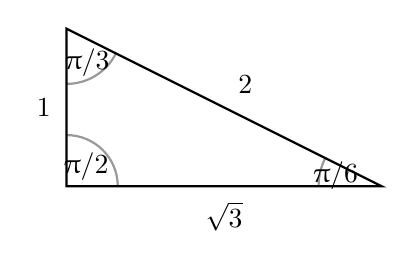
\begin{tikzpicture}[thick]
\coordinate (O) at (0,0);
\coordinate (A) at (4,0);
\coordinate (B) at (0,2);
\draw (O)--(A)--(B)--cycle;

\tkzLabelSegment[below=2pt](O,A){$\sqrt{3}$}
\tkzLabelSegment[left=2pt](O,B){$1$}
\tkzLabelSegment[above right=2pt](A,B){2}

\tkzMarkAngle[fill= orange,size=0.65cm,%
opacity=.4](A,O,B)
\tkzLabelAngle[pos = 0.35](A,O,B){$\uppi/2$}

\tkzMarkAngle[fill= orange,size=0.8cm,%
opacity=.4](B,A,O)
\tkzLabelAngle[pos = 0.6](B,A,O){$\uppi/6$}

\tkzMarkAngle[fill= orange,size=0.7cm,%
opacity=.4](O,B,A)
\tkzLabelAngle[pos = 0.5](O,B,A){$\uppi/3$}



\end{tikzpicture}
\end{multicols*}
%\newpage
\begin{multicols*}{2}
\subsection*{The 45-45-90 triangle}


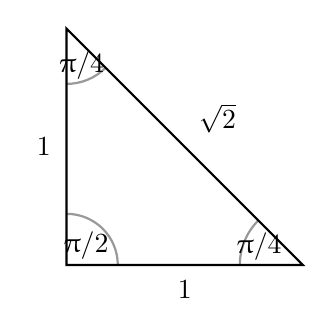
\begin{tikzpicture}[thick]
\coordinate (O) at (0,0);
\coordinate (A) at (3,0);
\coordinate (B) at (0,3);
\draw (O)--(A)--(B)--cycle;

\tkzLabelSegment[below=2pt](O,A){$1$}
\tkzLabelSegment[left=2pt](O,B){$1$}
\tkzLabelSegment[above right=2pt](A,B){$\sqrt{2}$}
\tkzMarkAngle[fill= orange,size=0.65cm,%
opacity=.4](A,O,B)
\tkzLabelAngle[pos = 0.35](A,O,B){$\uppi/2$}

\tkzMarkAngle[fill= orange,size=0.8cm,%
opacity=.4](B,A,O)
\tkzLabelAngle[pos = 0.6](B,A,O){$\uppi/4$}

\tkzMarkAngle[fill= orange,size=0.7cm,%
opacity=.4](O,B,A)
\tkzLabelAngle[pos = 0.5](O,B,A){$\uppi/4$}


\end{tikzpicture}

\section*{Laws of Cosine \& Sine}
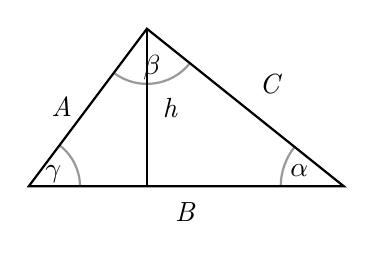
\begin{tikzpicture}[thick]
\coordinate (O) at (0,0);
\coordinate (A) at (4,0);
\coordinate (B) at (1.5,2);
\coordinate (C) at (1.5,0);
\draw (O)--(A)--(B)--cycle;
\draw (C)--(B)--cycle;

\tkzLabelSegment[below=2pt](O,A){\textit{B}}
\tkzLabelSegment[left=2pt](O,B){\textit{A}}
\tkzLabelSegment[above right=2pt](A,B){\textit{C}}
\tkzLabelSegment[right=2pt](C,B){\textit{h}}
\tkzMarkAngle[fill= orange,size=0.65cm,%
opacity=.4](A,O,B)
\tkzLabelAngle[pos = 0.35](A,O,B){$\gamma$}

\tkzMarkAngle[fill= orange,size=0.8cm,%
opacity=.4](B,A,O)
\tkzLabelAngle[pos = 0.6](B,A,O){$\alpha$}

\tkzMarkAngle[fill= orange,size=0.7cm,%
opacity=.4](O,B,A)
\tkzLabelAngle[pos = 0.5](O,B,A){$\beta$}


\end{tikzpicture}

\textbf{Law of cosine:} \,
\(
    C^2 = A^2 + B^2 - 2 A B \cos(\gamma) 
\)

\textbf{Law of sines:} \,
\(
    \frac{\sin(\alpha)}{A} =  \frac{\sin(\beta)}{B} =  \frac{\sin(\gamma)}{C}
\)

\textbf{Area:} \,
\(
    \mbox{Area} = \frac{1}{2} hB =   \frac{1}{2} A B \sin(\gamma)
\)

\section*{Hyperbolic Functions}
\vspace{-0.3in}
\begin{align*}
  &2 \cosh(x) = \exp(x) + \exp(-x) \\
  &2 \sinh(x) = \exp(x) - \exp(-x) \\
  & \tanh(x) = \nicefrac{\cosh(x)}{\sinh(x)}\\
  &\cosh(x)^2 - \sinh(x)^2 = 1
\end{align*}
\section*{Volumes}

\begin{comment}
\subsection*{Rectangle}
\begin{minipage}[c]{0.333\textwidth}
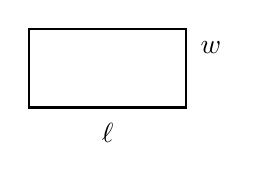
\begin{tikzpicture}[thick]
\coordinate (O) at (0,0);
\coordinate (A) at (2,0);
\coordinate (B) at (2,1);
\coordinate (C) at (0,1);
\draw (O)--(A)--(B)--(C)--cycle;

\tkzLabelSegment[below=2pt](O,A){$\ell$}
\tkzLabelSegment[above right=2pt](A,B){$w$}


\end{tikzpicture}

\[
   \mbox{Area} = \ell \times w
\]
\[
   \mbox{Perimeter} = 2 \ell  +  2 w
\]

\end{minipage}
\subsection*{Circle}

\[
   \mbox{Area} = \uppi  \times \mbox{radius}^2
\]
\[
   \mbox{Circumference} = 2 \uppi  \times \mbox{radius}
\]
\end{comment}
\subsection*{Right Circular Cylinder}

\begin{minipage}[c]{0.25\textwidth}
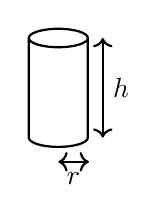
\begin{tikzpicture}[thick]
  \node (a) [cylinder, shape border rotate=90, draw, minimum height=15mm, minimum width=7.5mm] {};
  \draw [<->] ([xshift=5pt]a.before bottom) -- ([xshift=5pt]a.after top) node [midway, right] {$h$};
  \draw [<->] ([yshift=-5pt]a.bottom) -- ([yshift=-5pt]a.bottom -| a.before bottom) node [midway, below] {$r$};
\end{tikzpicture}
\end{minipage}
\begin{minipage}[l]{0.25\textwidth}
\noindent \textbf{Volume:} \,
\(
    \mbox{V} = \uppi r^2 h
\)

\noindent \textbf{Area: }  (not including circular ends)\,
\(
   \mbox{A} = 2 \uppi r  h
\)
\end{minipage}
\subsection*{Cone} 
  \begin{minipage}[c]{0.25\textwidth}
   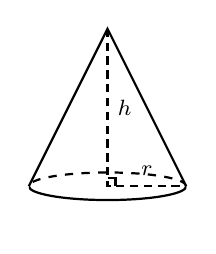
\begin{tikzpicture}[thick, scale=0.5]
      \begin{scope}
     \clip (-2,0) rectangle (2,1cm);
    \draw[dashed] (0,0) circle(2cm and 0.35cm);
    \end{scope}
    \begin{scope}
     \clip (-2,0) rectangle (2,-1cm);
    \draw (0,0) circle(2cm and 0.35cm);
    \end{scope}
    \draw[densely dashed] (0,4) -- node[right,font=\footnotesize] {$h$}coordinate[pos=0.95] (aa)(0,0)
                            -- node[above,font=\footnotesize] {$r$}coordinate[pos=0.1] (bb) (2,0);
    \draw (aa) -| (bb);
    \draw (-2,0) -- (0,4) -- (2,0);
  \end{tikzpicture}
  \end{minipage}
  \begin{minipage}[c]{0.25\textwidth}
  \noindent \textbf{Volume:} \,
  \(
     \mbox{V} = \frac{1}{3} \uppi r^2 h
  \)
  
\noindent \textbf{Area} (not including circular base) \, \\
\(
   \quad \mbox{A} =  \uppi r   \sqrt{r^2+h^2}
\)
\end{minipage}

\subsection*{Sphere}
\begin{minipage}[c]{0.25\textwidth}
\(\phantom{xxx}\)
\end{minipage}
\begin{minipage}[c]{0.25\textwidth}
\noindent  \textbf{Area:}   \(A = 4 \uppi   r^2 \)

\noindent  \textbf{Volume:}   \(V = \frac{4 \uppi}{3} r^3 \)
\end{minipage}

\vfill

\section*{Unit Circle}

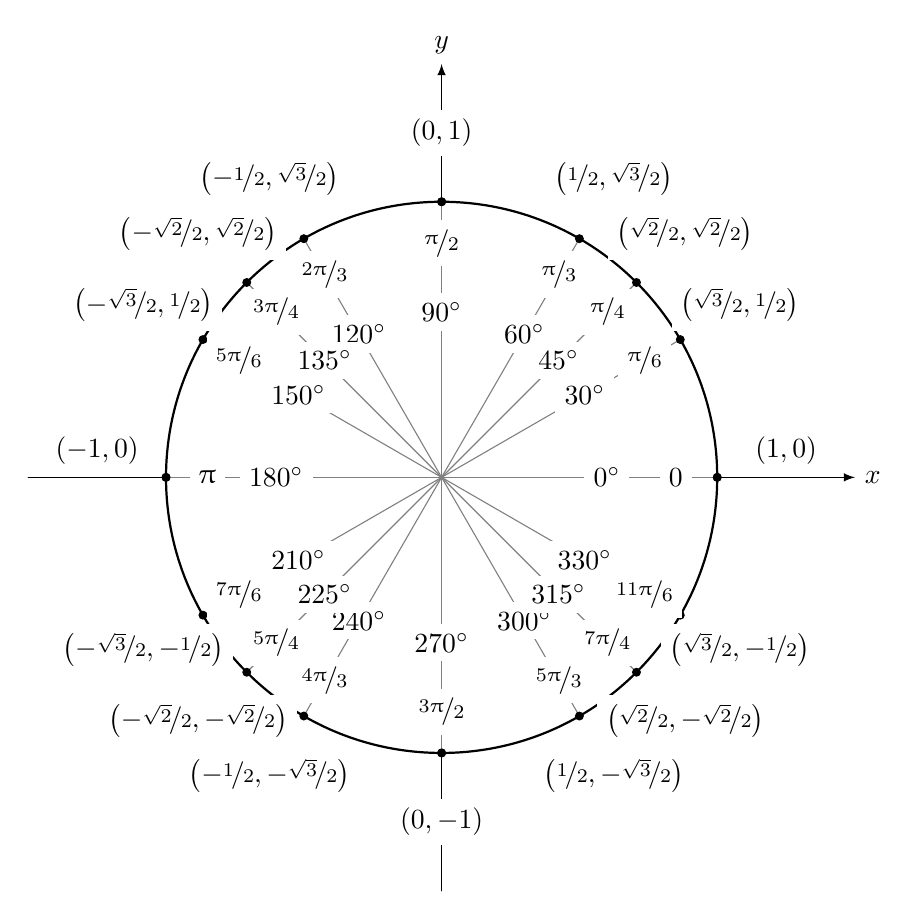
\begin{tikzpicture}[scale=3.5,cap=round,>=latex]
    % draw the coordinates
    \draw[->] (-1.5cm,0cm) -- (1.5cm,0cm) node[right,fill=white] {$x$};
    \draw[->] (0cm,-1.5cm) -- (0cm,1.5cm) node[above,fill=white] {$y$};

    % draw the unit circle
    \draw[thick] (0cm,0cm) circle(1cm);

    \foreach \x in {0,30,...,330} {
            % lines from center to point
            \draw[gray] (0cm,0cm) -- (\x:1cm);
            % dots at each point
            \filldraw[black] (\x:1cm) circle(0.4pt);
            % draw each angle in degrees
            \draw (\x:0.6cm) node[fill=white] {$\x^\circ$};
    }

    \foreach \x in {0,45,...,315} {
            % lines from center to point
            \draw[gray] (0cm,0cm) -- (\x:1cm);
            % dots at each point
            \filldraw[black] (\x:1cm) circle(0.4pt);
            % draw each angle in degrees
            \draw (\x:0.6cm) node[fill=white] {$\x^\circ$};
    }

    % draw each angle in radians
    \foreach \x/\xtext in {
        30/\nicefrac{\uppi}{6},
        45/\nicefrac{\uppi}{4},
        60/\nicefrac{\uppi}{3},
        90/\nicefrac{\uppi}{2},
        120/\nicefrac{2\uppi}{3},
        135/\nicefrac{3\uppi}{4},
        150/\nicefrac{5\uppi}{6},
        180/\uppi,
        210/\nicefrac{7\uppi}{6},
        225/\nicefrac{5\uppi}{4},
        240/\nicefrac{4\uppi}{3},
        270/\nicefrac{3\uppi}{2},
        300/\nicefrac{5\uppi}{3},
        315/\nicefrac{7\uppi}{4},
        330/\nicefrac{11\uppi}{6},
        0/0}
            \draw (\x:0.85cm) node[fill=white] {$\xtext$};

    \foreach \x/\xtext/\y in {
        % the coordinates for the first quadrant
        30/\nicefrac{\sqrt{3}}{2}/\nicefrac{1}{2},
        45/\nicefrac{\sqrt{2}}{2}/\nicefrac{\sqrt{2}}{2},
        60/\nicefrac{1}{2}/\nicefrac{\sqrt{3}}{2},
        % the coordinates for the second quadrant
        150/-\nicefrac{\sqrt{3}}{2}/\nicefrac{1}{2},
        135/-\nicefrac{\sqrt{2}}{2}/\nicefrac{\sqrt{2}}{2},
        120/-\nicefrac{1}{2}/\nicefrac{\sqrt{3}}{2},
        % the coordinates for the third quadrant
        210/-\nicefrac{\sqrt{3}}{2}/-\nicefrac{1}{2},
        225/-\nicefrac{\sqrt{2}}{2}/-\nicefrac{\sqrt{2}}{2},
        240/-\nicefrac{1}{2}/-\nicefrac{\sqrt{3}}{2},
        % the coordinates for the fourth quadrant
        330/\nicefrac{\sqrt{3}}{2}/-\nicefrac{1}{2},
        315/\nicefrac{\sqrt{2}}{2}/-\nicefrac{\sqrt{2}}{2},
        300/\nicefrac{1}{2}/-\nicefrac{\sqrt{3}}{2}}
            \draw (\x:1.25cm) node[fill=white] {$\left(\xtext,\y\right)$};

    % draw the horizontal and vertical coordinates
    % the placement is better this way
    \draw (-1.25cm,0cm) node[above=1pt] {$(-1,0)$}
          (1.25cm,0cm)  node[above=1pt] {$(1,0)$}
          (0cm,-1.25cm) node[fill=white] {$(0,-1)$}
          (0cm,1.25cm)  node[fill=white] {$(0,1)$};
\end{tikzpicture}
\section*{Applications}
Arclength of curve \(y = f(x)\) with \(a \leq x \leq b\)
\[
   = \int_a^b \sqrt{1 + f^\prime(x)^2} \, \mathrm{d} x
\]
For the region \(Q\) of the xy plane given by
\[
   Q = \{(x,y) \mid f(x) \leq y \leq g(x) \land a \leq x \leq b \},
\]
we have
\[
  \mbox{Area}(Q) = \int_a^b g(x) - f(x) \, \mathrm{d} x
\]  
Assuming \(0 \leq f(x)\) and rotating about the \mbox{x-axis}
\[
  \mbox{Vol}(Q) = \uppi \int_a^b g(x)^2 - f(x)^2 \, \mathrm{d} x
\]
Assuming \(0 \leq a < b\) and rotating about the y-axis
\[
  \mbox{Vol}(Q) = 2 \uppi \int_a^b x (g(x)  - f(x)) \, \mathrm{d} x
\]
Centroid
\begin{align*}
    \mbox{Area}(Q) \times \overline{x} &=  \int_a^b x \left(g(x) - f(x) \right) \, \mathrm{d} x \\
     \mbox{Area}(Q) \times \overline{y} &=  \frac{1}{2} \int_a^b  \left (g(x)^2  - f(x)^2 \right) \, \mathrm{d} x
\end{align*}
For the region \(Q\) of the xy plane given by
\[
   Q = \{(x,y) \mid f(y) \leq x \leq g(y) \land a \leq y \leq b \},
\]
interchange \(x\) and \(y\) in \emph{all} the previous formulas. 
\begin{comment}
Specifically
we have
\[
  \mbox{Area}(Q) = \int_a^b g(y) - f(y) \, \mathrm{d} y
\]  
Assuming \(0 \leq f(y)\) and rotating about the \mbox{y-axis}
\[
  \mbox{Vol}(Q) = \uppi \int_a^b g(y)^2 - f(y)^2 \, \mathrm{d} y
\]
Assuming \(a \geq 0\) and rotating about the x-axis
\[
  \mbox{Vol}(Q) = 2 \uppi \int_a^b y (g(y)  - f(y)) \, \mathrm{d} y
\]
Centroid
\begin{align*}
    \mbox{Area}(Q) \times \overline{y} &=  \int_a^b y \left(g(y) - f(y) \right) \, \mathrm{d} y \\
     \mbox{Area}(Q) \times \overline{x} &=  \frac{1}{2} \int_a^b  \left (g(y)^2  - f(y)^2 \right) \, \mathrm{d} y
\end{align*}
\end{comment}
\vfill 

%To view a copy of this license, visit \url{https://creativecommons.org/publicdomain/zero/1.0 }
%\vspace{0.25in}
%\tiny
\noindent Revised \today. Barton Willis is the author of this work. This work is
licensed under Attribution 4.0 International (CC BY 4.0) \,  \qrcode[height=0.15in]{https://creativecommons.org/licenses/by/4.0/}. For the current version of
this document, visit \, \qrcode[height=0.15in]{https://github.com/barton-willis/Calculus-I-} 

\end{multicols*}

\end{document}